\documentclass[12pt]{article}
\usepackage[a4paper]{geometry}
\usepackage{fullpage}
\usepackage[T1]{fontenc}
\usepackage[utf8]{inputenc}
\usepackage{graphicx}
\usepackage{mathpazo}
\pagenumbering{gobble}
\usepackage{siunitx}
\DeclareSIUnit\voltampere{VA}
\usepackage{amsmath}
\usepackage[spanish]{babel}
\usepackage{steinmetz}
\usepackage{enumitem}
\renewcommand{\thesection}{Problema \arabic{section}}

\begin{document}

\title{}

\date{2019-20}

\section{}

Un sistema trifásico de secuencia de fases inversa y tensión
$\SI[parse-numbers=false]{200\sqrt{3}}{\volt}$, alimenta a tres
impedancias iguales de valor
$\overline{Z} = \SI[parse-numbers=false]{10\phase{\ang{60}}}{\ohm}$,
conectadas en estrella. Determina la corriente de línea.

\noindent\hrulefill

\[ U = \SI[parse-numbers=false]{200\sqrt{3}}{\volt} \rightarrow U_f =
  \SI{200}{\volt}
\]
\begin{align*} \overline{U}_A &=
                                \SI[parse-numbers=false]{200\phase{\ang{-90}}}{\volt}\\
  \overline{U}_B
                              &= \SI[parse-numbers=false]{200\phase{\ang{30}}}{\volt}\\
  \overline{U}_C &=
                   \SI[parse-numbers=false]{200\phase{\ang{150}}}{\volt}\\
\end{align*}

\begin{align*} \overline{I}_A &= \frac{\overline{U}_A}{\overline{Z}} =
  \frac{200}{10}\phase{\ang{-90} - \ang{60}} \\ \overline{I}_B &=
  \frac{\overline{U}_B}{\overline{Z}} = \frac{200}{10}\phase{\ang{30}
    - \ang{60}}\\ \overline{I}_C &=
  \frac{\overline{U}_C}{\overline{Z}} = \frac{200}{10}\phase{\ang{150}
    - \ang{60}}
\end{align*}

\begin{align*} \overline{I}_A &=
                                \SI[parse-numbers=false]{20\phase{\ang{-150}}}{\ampere}\\
  \overline{I}_B &=
                   \SI[parse-numbers=false]{20\phase{\ang{-30}}}{\ampere}\\
  \overline{I}_C &=
                   \SI[parse-numbers=false]{20\phase{\ang{90}}}{\ampere}
\end{align*}

\[ \overline{I}_A + \overline{I}_B + \overline{I}_C = 0
\]

\clearpage
 
\section{}

Un sistema trifásico de secuencia de fases directa y tensión
$\SI{200}{\volt}$ alimenta tres impedancias iguales de valor
$\overline{Z} = \SI[parse-numbers=false]{10\phase{\ang{30}}}{\ohm}$,
conectadas en triángulo. Determina las corrientes de fase y línea.

\noindent\hrulefill

\[
  U = \SI[parse-numbers=false]{200}{\volt}
\]
  
  \begin{align*}
    \overline{U}_{AB} &= \SI[parse-numbers=false]{200\phase{\ang{120}}}{\volt}\\
    \overline{U}_{BC} &= \SI[parse-numbers=false]{200\phase{\ang{0}}}{\volt}\\
    \overline{U}_{CA} &= \SI[parse-numbers=false]{200\phase{\ang{-120}}}{\volt}\\
  \end{align*}

 \begin{align*}
   \overline{I}_{AB} &= \frac{\overline{U}_{AB}}{\overline{Z}} = \frac{200}{10}\phase{\ang{120} - \ang{30}} \\
   \overline{I}_{BC} &= \frac{\overline{U}_{BC}}{\overline{Z}} = \frac{200}{10}\phase{\ang{0} - \ang{30}}\\
   \overline{I}_{CA} &= \frac{\overline{U}_{CA}}{\overline{Z}} = \frac{200}{10}\phase{\ang{-120} - \ang{30}}
 \end{align*}

  \begin{align*}
    \overline{I}_{AB} &= \SI[parse-numbers=false]{20\phase{\ang{90}}}{\ampere}\\
    \overline{I}_{BC} &= \SI[parse-numbers=false]{20\phase{\ang{-30}}}{\ampere}\\
    \overline{I}_{CA} &= \SI[parse-numbers=false]{20\phase{\ang{-150}}}{\ampere}
  \end{align*}

 \begin{align*}
   \overline{I}_A &= \overline{I}_{AB} - \overline{I}_{CA} = \SI[parse-numbers=false]{20\sqrt{3}\phase{\ang{90}-\ang{30}}}{\ampere}=  \SI[parse-numbers=false]{20\sqrt{3}\phase{\ang{60}}}{\ampere}\\
   \overline{I}_B &= \overline{I}_{BC} - \overline{I}_{AB} = \SI[parse-numbers=false]{20\sqrt{3}\phase{\ang{-30} - \ang{30}}}{\ampere} =  \SI[parse-numbers=false]{20\sqrt{3}\phase{\ang{-60}}}{\ampere}\\
   \overline{I}_C &= \overline{I}_{CA} - \overline{I}_{BC} = \SI[parse-numbers=false]{20\sqrt{3}\phase{\ang{-150} - \ang{30}}}{\ampere}=  \SI[parse-numbers=false]{20\sqrt{3}\phase{\ang{-180}}}{\ampere}\\
 \end{align*}

 \clearpage
 
\section{}
Un sistema trifásico de cuatro conductores, de secuencia de fases
directa y $\SI[parse-numbers=false]{200\sqrt{3}}{\volt}$ alimenta a
tres impedancias:
$\overline{Z}_{A} =
\SI[parse-numbers=false]{10\phase{\ang{60}}}{\ohm}$,
$\overline{Z}_{B} = \SI[parse-numbers=false]{10\phase{\ang{0}}}{\ohm}$
y
$\overline{Z}_{C} =
\SI[parse-numbers=false]{10\phase{\ang{-30}}}{\ohm}$. Determina las
corrientes de línea.

\noindent\hrulefill

\[ U = \SI[parse-numbers=false]{200\sqrt{3}}{\volt} \rightarrow U_f =
  \SI{200}{\volt}
\]
\begin{align*}
  \overline{U}_A &= \SI[parse-numbers=false]{200\phase{\ang{90}}}{\volt}\\
  \overline{U}_B &= \SI[parse-numbers=false]{200\phase{\ang{-30}}}{\volt}\\
  \overline{U}_C &= \SI[parse-numbers=false]{200\phase{\ang{-150}}}{\volt}\\
\end{align*}

\begin{align*}
  \overline{I}_A &= \frac{\overline{U}_A}{\overline{Z}} = \frac{200}{10}\phase{\ang{90} - \ang{60}} \\
  \overline{I}_B &= \frac{\overline{U}_B}{\overline{Z}} = \frac{200}{10}\phase{\ang{-30} - \ang{0}}\\
  \overline{I}_C &= \frac{\overline{U}_C}{\overline{Z}} = \frac{200}{10}\phase{\ang{-150} - (\ang{-30})}
\end{align*}

 \begin{align*}
   \overline{I}_A &= \SI[parse-numbers=false]{20\phase{\ang{30}}}{\ampere}\\
   \overline{I}_B &= \SI[parse-numbers=false]{20\phase{\ang{-30}}}{\ampere}\\
   \overline{I}_C &= \SI[parse-numbers=false]{20\phase{\ang{-120}}}{\ampere}
 \end{align*}

 \[
   \overline{I}_N = -(\overline{I}_A + \overline{I}_B +
   \overline{I}_C) =
   \SI[parse-numbers=false]{30.12\phase{\ang{144.89}}}{\ampere}
 \]

 \clearpage
 
 \section{}

 Un sistema trifásico de secuencia de fases inversa y tensión
 $\SI{200}{\volt}$, alimenta a tres impedancias que son:
 $\overline{Z}_{AB} =
 \SI[parse-numbers=false]{10\phase{\ang{0}}}{\ohm}$,
 $\overline{Z}_{BC} =
 \SI[parse-numbers=false]{10\phase{\ang{30}}}{\ohm}$ y
 $\overline{Z}_{CA} =
 \SI[parse-numbers=false]{10\phase{\ang{-45}}}{\ohm}$, conectadas en
 triángulo. Determina las corrientes de fase y línea.

 \noindent\hrulefill
 
\[
  U = \SI[parse-numbers=false]{200}{\volt}
\]
  
  \begin{align*}
    \overline{U}_{AB} &= \SI[parse-numbers=false]{200\phase{\ang{-120}}}{\volt}\\
    \overline{U}_{BC} &= \SI[parse-numbers=false]{200\phase{\ang{0}}}{\volt}\\
    \overline{U}_{CA} &= \SI[parse-numbers=false]{200\phase{\ang{120}}}{\volt}\\
  \end{align*}

 \begin{align*}
   \overline{I}_{AB} &= \frac{\overline{U}_{AB}}{\overline{Z}} = \frac{200}{10}\phase{\ang{-120} - \ang{0}} \\
   \overline{I}_{BC} &= \frac{\overline{U}_{BC}}{\overline{Z}} = \frac{200}{10}\phase{\ang{0} - \ang{30}}\\
   \overline{I}_{CA} &= \frac{\overline{U}_{CA}}{\overline{Z}} = \frac{200}{10}\phase{\ang{120} - \ang{-45}}
 \end{align*}

  \begin{align*}
    \overline{I}_{AB} &= \SI[parse-numbers=false]{20\phase{\ang{-120}}}{\ampere}\\
    \overline{I}_{BC} &= \SI[parse-numbers=false]{20\phase{\ang{-30}}}{\ampere}\\
    \overline{I}_{CA} &= \SI[parse-numbers=false]{20\phase{\ang{165}}}{\ampere}
  \end{align*}

 \begin{align*}
   \overline{I}_A &= \overline{I}_{AB} - \overline{I}_{CA} = \SI[parse-numbers=false]{24.35\phase{\ang{-67.5}}}{\ampere}\\
   \overline{I}_B &= \overline{I}_{BC} - \overline{I}_{AB} = \SI[parse-numbers=false]{28.28\phase{\ang{15}}}{\ampere}\\
   \overline{I}_C &= \overline{I}_{CA} - \overline{I}_{BC} = \SI[parse-numbers=false]{39.66\phase{\ang{157.5}}}{\ampere}\\
 \end{align*}

 \clearpage
 
 \section{}

 Una plantación agrícola emplea dos bombas sumergibles para extraer
 agua de un pozo y transportarla a través de un sistema de riego por
 goteo. Estas dos bombas están alimentadas a \SI{400}{\volt} por una
 línea trifásica en secuencia de fases directa y frecuencia
 $\SI{50}{\hertz}$. Una de las bombas funciona con un motor trifásico
 de $\SI{30}{\kilo\watt}$ y factor de potencia de 0.78. La otra bomba
 trabaja con un motor de $\SI{7.5}{\kilo\watt}$ y factor de potencia
 de 0.67.  La línea que alimenta estas dos bombas es resistiva, con
 resistividad $\rho = \SI{0.017}{\ohm\milli\meter\squared\per\meter}$,
 longitud de \SI{300}{m} y una sección de
 \SI{35}{\milli\meter\squared}.
 
 \begin{enumerate}
 \item Calcula el triángulo de potencias (potencia activa, reactiva, y
   aparente) de cada carga, y total de las cargas (a la salida de la
   línea).
 \item Calcula el \textbf{valor eficaz} de la corriente de línea de
   cada carga, y total.
 \item Determine la lectura de los siguientes aparatos de medida
   conectados a la entrada de las cargas:
   \begin{itemize}
   \item Un vatímetro en la fase A, midiendo tensión entre las fases A
     y C.
   \item Un vatímetro en la fase B, midiendo tensión entre las fases B
     y C.
   \item Un vatímetro en la fase C, midiendo tensión entre las fases B
     y A.
   \end{itemize}
 \item Calcule el triángulo de potencias a la entrada de la línea.
 \item Calcule el \textbf{valor eficaz} de la tensión a la entrada de la línea.
 \item Calcule los condensadores que se deben conectar a la salida de
   la línea para mejorar el factor de potencia del sistema hasta la
   unidad. Indique el modo de conexión.
 \end{enumerate}

Una vez conectados los condensadores del último apartado:
\begin{enumerate}[resume]
\item Calcule el \textbf{valor eficaz} de la corriente de línea total.
\item Calcule el triángulo de potencias a la entrada de la línea.
\item Calcule el \textbf{valor eficaz} de la tensión a la entrada de la línea.
\item Determine la lectura de los vatímetros descritos anteriormente.
\end{enumerate}

\noindent\hrulefill

 Las potencias de cada carga son:
 \begin{align*}
   P_1 &= \SI{30}{\kilo\watt}\\
   Q_1 &= P_1\tan \theta_1 = \SI{24.06}{\kilo\voltampere}_r\\
   S_1 &= \SI{38.46}{\kilo\voltampere}\\
   P_2 &= \SI{7.5}{\kilo\watt}\\
   Q_2 &= P_2 \tan \theta_2 = \SI{8.31}{\kilo\voltampere}_r\\
   S_2 &= \SI{11.19}{\kilo\voltampere}
 \end{align*}

 Aplicando Boucherot, el triángulo de potencias total es:
 \begin{align*}
   P_T &= \SI{37.5}{\kilo\watt}\\
   Q_T &= \SI{32.37}{\kilo\voltampere}_r\\
   S_T &= \sqrt{P_T^2 + Q_T^2} = \SI{49.54}{\kilo\voltampere}
 \end{align*}

 Por tanto, el ángulo de la impedancia global es:

\[
  \tan(\theta) = \frac{Q_T}{P_T} = 0.8632 \rightarrow \theta =
  \ang{40.8}
\]

Las corrientes en cada carga son:

\begin{align*}
  I_1 &= \frac{S_1}{\sqrt{3} U} = \SI{55.51}{\ampere}\\
  I_2 &= \frac{S_2}{\sqrt{3} U} = \SI{16.15}{\ampere}
\end{align*}

La corriente total es:
\[
  I = S_T /{\sqrt{3} U} = \SI{71.5}{\ampere}
\]

Denominaremos con $W_1$ al vatímetro conectado en la fase A midiendo
tensión entre las fases A y C, y con $W_2$ al vatímetro conectado en
la fase B midiendo tensión entre las fases B y C. Teniendo en cuenta
que se trata de una SFD:
 
\begin{align*}
  W_1 + W_2 &= P_T\\
  W_1 - W_2 &= Q_T/\sqrt{3}
\end{align*}

Por tanto:

\begin{align*}
  W_1 &= 1/2 (P_T + Q_T/\sqrt{3}) = \SI{28.09}{\kilo\watt}\\
  W_2 &= 1/2 (P_T - Q_T/\sqrt{3}) = \SI{9.41}{\kilo\watt}
\end{align*}

También podemos obtener estos resultados con las siguientes
ecuaciones:

\begin{align*}
  W_1 &= U I \cos(\theta - \ang{30}) = \SI{28.09}{\kilo\watt}\\
  W_2 &= U I \cos(\theta + \ang{30}) = \SI{9.41}{\kilo\watt}
\end{align*}

Por otra parte, el vatímetro de la fase C mide:

\[
  W_{C, BA} = - \frac{Q_T}{\sqrt{3}} = - \SI{18.66}{\kilo\watt}
\]

La resistencia de la línea (una resistencia por cada conductor) es:

\[
R_L = \rho L/S = \SI{0.146}{\ohm}
\]

La potencia activa disipada en la línea es:

\[
P_L = 3 \cdot I^2 R_L = \SI{2234.8}{\watt}
\]

Por tanto, la potencia a la entrada de la línea es:

\begin{align*}
P_g &= P_L + P_T = \SI{39.73}{\kilo\watt}\\
Q_g &= Q_T = \SI{32.33}{\kilo\voltampere}_r\\
S_g &= \SI{51.22}{\kilo\voltampere}
\end{align*}

Y la tensión a la salida del generador (entrada de la línea) es:

\[
U_g = \frac{S_g}{\sqrt{3} I} = \SI{413.64}{\volt}
\]

Para mejorar el factor de potencia a la unidad en las cargas, se necesita una batería de condensadores conectados en triángulo en las cargas (a la salida de la línea). Cada uno de los tres condensadores debe tener una capacidad de:

\[
C = \frac{Q_T}{3 \omega V^2} = \SI{214.4}{\micro\farad}
\]

Una vez instalada la batería de condensadores, la corriente total a la salida de la línea es:

\[
I' = \frac{P_T}{\sqrt{3} U} = \SI{54.13}{\ampere}
\]

La potencia disipada en la línea es ahora:

\[
P'_L = 3 \cdot I'^2 R_L = \SI{1282.9}{\watt} 
\]

Por tanto, el triángulo de potencias a la entrada de la línea es:
\begin{align*}
P'_g &= \SI{38.78}{\kilo\watt}\\
Q'_g &= \SI{0}{\kilo\voltampere}_r\\
S'_g &= \SI{38.78}{\kilo\voltampere}
\end{align*}

Consecuentemente, la tensión a la entrada de la línea es:

\[
U' = \frac{S'_g}{\sqrt{3} I'} = \SI{413.63}{\volt}
\]

Con la inserción de los condensadores los vatímetros miden:

\begin{align*}
W'_{A, AC} = W'_{B, BC} &= 1/2 \cdot P'_T = \SI{18.75}{\kilo\watt}\\
W'_{C, BA} &= \SI{0}{\watt}
\end{align*}

\clearpage

\section{}

El circuito de la figura es de secuencia de fases directa y 50 Hz. Determinar:
\begin{enumerate}
\item Potencias activas y reactivas totales.
\item Capacidad mínima de los condensadores a instalar para mejorar el factor de potencia total hasta la unidad.
\item Intensidades de línea, en forma fasorial, una vez mejorado el factor de potencia.
\end{enumerate}
Datos: 

\begin{align*}
  \overline{Z}_1 &= \SI[parse-numbers=false]{100\phase{\ang{60}}}{\ohm}\\
  W_1 &= \SI{300}{\watt}\\
  W_2 &= \SI{300}{\watt}\\
  V &= \SI[parse-numbers=false]{\sqrt{3} \cdot 200}{\volt}
\end{align*}

\begin{center}
  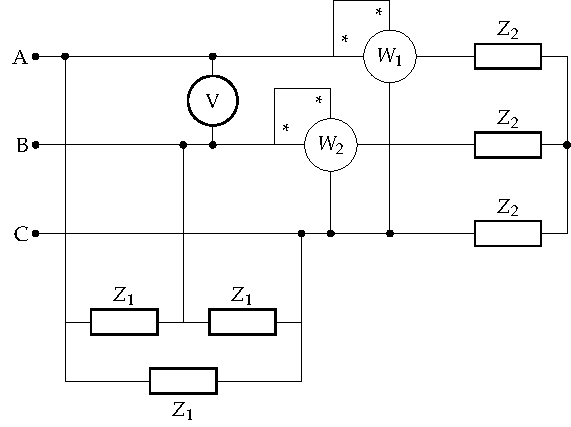
\includegraphics{figs/ZyZt}
\end{center}

\noindent\hrulefill

Los dos vatímetros miden la potencia de la impedancia $Z_2$:

\begin{align*}
  P_2 &= W_1 + W_2 = \SI{600}{\watt}\\
  Q_2 &= \sqrt{3}\cdot (W_1 - W_2) = \SI{0}{\volt\ampere_r}
\end{align*}

Para calcular la potencia de $Z_2$ debemos obtener la corriente de fase:

\[
  I_{1f} = \frac{U}{Z_1} = \SI[parse-numbers=false]{2\sqrt{3}}{\ampere}
\]

Por tanto,

\begin{align*}
  P_2 &= 3 \cdot I_{1f}^2 R_1 = 3 \cdot (2\sqrt{3})^2 \cdot (100\cos(\ang{60})) = \SI{1800}{\watt}\\
  Q_2 &= 3 \cdot I_{1f}^2 X_1 = 3 \cdot (2\sqrt{3})^2 \cdot (100\sin(\ang{60})) = \SI[parse-numbers=false]{1800\sqrt{3}}{\volt\ampere_r}
\end{align*}

Aplicando Boucherot:

\begin{align*}
  P &= P_1 + P_2 = \SI{2400}{\watt}\\
  Q &= Q_1 + Q_2 = \SI[parse-numbers=false]{1800\sqrt{3}}{\volt\ampere_r}
\end{align*}

Se deben instalar tres condensadores en triángulo con capacidad:

\[
  C_\triangle = \frac{Q}{3 \cdot \omega U^2} = \SI{27.57}{\micro\farad}
\]

Al instalar estos condensadores la corriente que circula por la línea es:

\[
  P = \sqrt{3} \cdot U \cdot I' \rightarrow I' = \SI{4}{\ampere}
\]

En forma fasorial, teniendo en cuenta que $\theta' = \ang{0}$:

\begin{align*}
  \overline{I}_A &= \SI[parse-numbers=false]{4\phase{\ang{90}}}{\ampere}\\
  \overline{I}_B &= \SI[parse-numbers=false]{4\phase{\ang{-30}}}{\ampere}\\
  \overline{I}_C &= \SI[parse-numbers=false]{4\phase{\ang{-150}}}{\ampere}
\end{align*}

\clearpage



\section{}

En la figura dos vatímetros miden una carga trifásica inductiva
equilibrada alimentada a una tensión $U = \SI{400}{\volt}$. El
vatímetro $W_B$ indica una lectura de \SI{11320}{\watt}, y el
vatímetro $W_C$ indica una lectura de \SI{1815}{\watt}. A partir de
esta información se pide:

\begin{enumerate}
\item Determinar la secuencia de fases del sistema.
\item Triángulo de potencias de la carga.
\item Impedancia equivalente de la carga en estrella y
  en triángulo.
\item Tensión de alimentación a la entrada de la línea
  $U_1$ sabiendo que la línea de alimentación es resistiva pura con
  valor $R = \SI{0.1}{\ohm}$.
\item Capacidad de los condensadores que se deben
  conectar en bornes de la carga para conseguir mejorar su factor de
  potencia a la unidad. Determinar las nuevas lecturas de los
  vatímetros $W_B$ y $W_c$.
\end{enumerate}

\begin{center}
  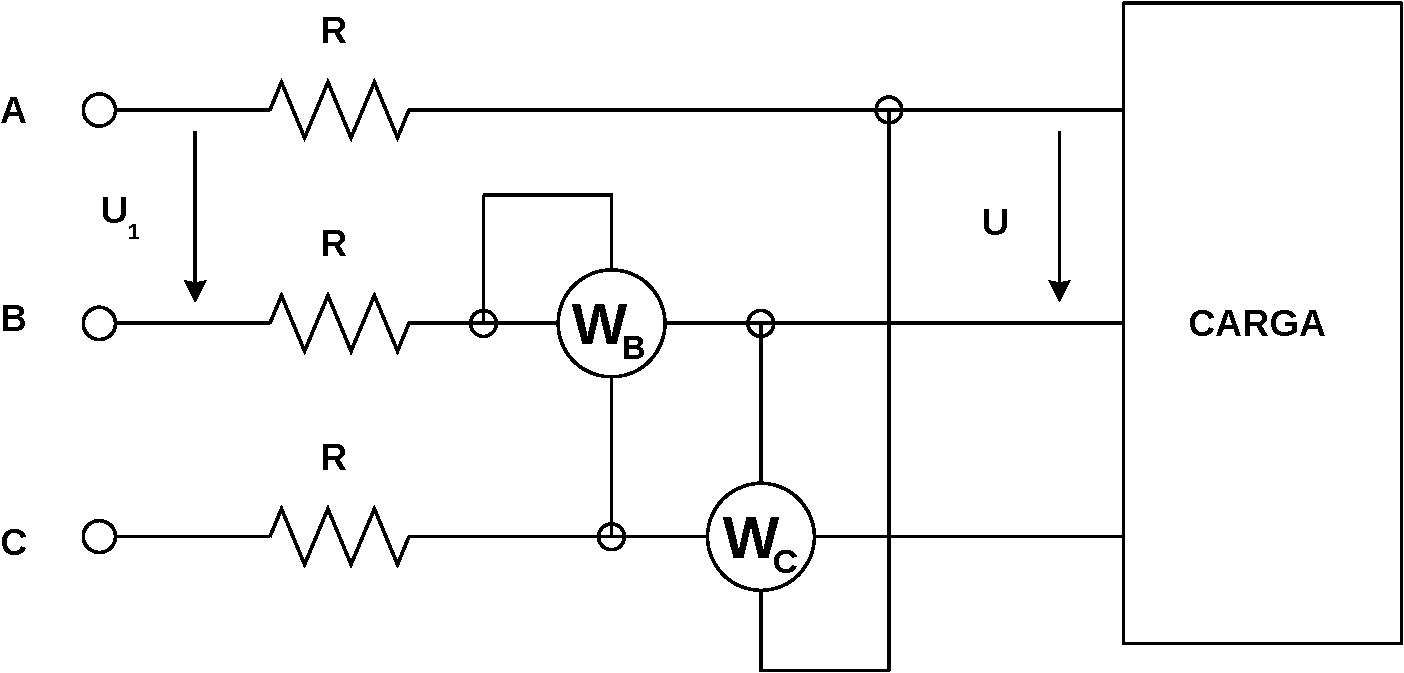
\includegraphics[height=0.3\textheight]{figs/Esquema.pdf}
\end{center}

\noindent\hrulefill

El vatímetro $W_c$ está conectado de forma que mide la potencia
reactiva:

\[
  W_c = \pm \frac{Q}{\sqrt{3}}
\]

Dado que el vatímetro está conectado entre B y A, el signo negativo
corresponde a SFD y el positivo a SFI. Dado que la carga es inductiva
es $Q > 0$. Como $W_c > 0$ debemos elegir el signo positivo, lo que
implica SFI.

Al vatímetro $W_B$ podríamos añadirle un hipotético vatímetro
$W_A$ conectado en la fase A midiendo tensión entre A y C para
emplear el método de los dos vatímetros:


\begin{align*}
W_B + W_A &= P\\
W_B - W_A &= \frac{Q}{\sqrt{3}} = W_c
\end{align*}

Restando ambas ecuaciones obtenemos:

\[
  P = 2 W_B - W_c = \SI{20825}{\watt}
\]

La potencia reactiva se calcula directamente con el vatímetro $W_c$:

\[
  Q = \sqrt{3} W_c = \SI{3143.7}{VA}_r
\]

Por tanto:

\[
  \overline{S} =
  \SI[parse-numbers=false]{21060.9\phase{\ang{8.58}}}{VA}
\]

El módulo de la impedancia en triángulo se obtiene con
$Z_{\triangle} = U / I_f$. Teniendo en cuenta que $S = \sqrt{3} U I$
y que $I = \sqrt{3} I_f$, obtenemos $I_f = S / 3U$. Por tanto
\[
  \overline{Z}_{\triangle} = \frac{3 U^2}{S}\phase{\ang{8.58}} =
  \SI[parse-numbers=false]{22.8\phase{\ang{8.58}}}{\ohm}
\]


Para obtener la impedancia en estrella basta con usar las relaciones
entre tensiones y corrientes de fase y línea:

\begin{align*}
  Z_Y &= \frac{U_f}{I} = \frac{1}{\sqrt{3}} \cdot \frac{U}{I}\\
  Z_\triangle &= \frac{U}{I_f} = \sqrt{3} \cdot \frac{U}{I}
\end{align*}

Por tanto, $\overline{Z}_{Y} = \overline{Z}_{\triangle} / 3$.

La corriente de línea es:

\[
  I = \frac{S}{\sqrt{3} U} = \SI{30.4}{\ampere}
\]

La potencia disipada en la línea es:

\[
  P_L = 3 \cdot I^2 \cdot R_L = \SI{277.23}{\watt}
\]

La potencia aparente total a la entrada de la línea es:

\[
  S_T = \sqrt{(P + P_L)^2 + Q^2} = \SI{21335.1}{VA}
\]

Y, por tanto,

\[
  U_1 = \frac{S_T}{\sqrt{3} I} = \SI{405.21}{\volt}
\]

Suponiendo $f = \SI{50}{\hertz}$:
\[
  C = \frac{Q}{3 \omega U^2} = \SI{20.85}{\micro\farad}
\]

Ahora, dado que $Q' = \SI{0}{VA}_r$, será $W_C = \SI{0}{\watt}$ y
$W_B = P/2 = \SI{10412.5}{\watt}$.

\clearpage

\section{}

Del circuito de la figura se sabe que tiene una secuencia de fases
directa ABC. El amperímetro indica $\SI{5}{\ampere}$, el voltímetro
$\SI{400}{\volt}$, y los vatímetros A y C muestran una lectura
idéntica. Se pide:

\begin{enumerate}
\item Valor de la impedancia Z en forma compleja.
\item Expresión fasorial de todas las intensidades del circuito.
\item Lecturas de los vatímetros A y C.
\end{enumerate}

\begin{center}
  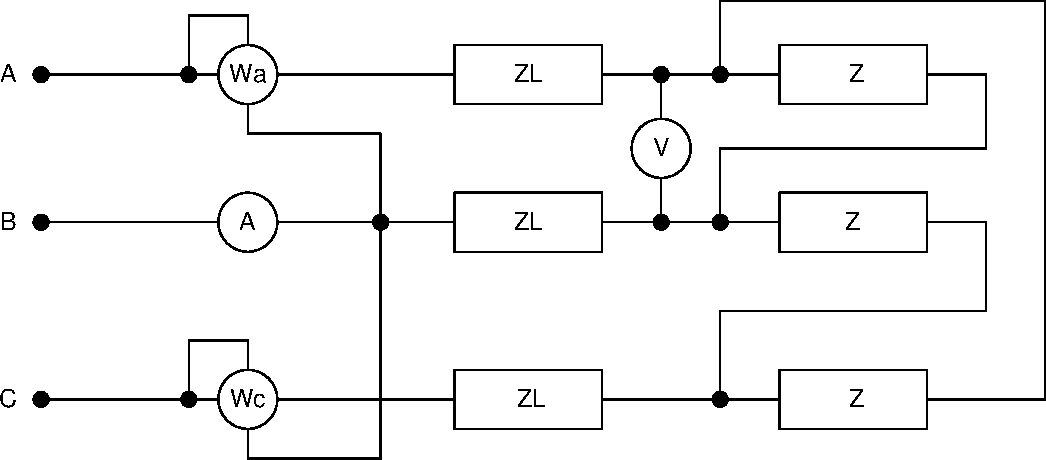
\includegraphics[width = 0.9\textwidth]{figs/trifasica}
\end{center}

Dato: $\overline{Z}_L = \SI[parse-numbers = false]{1 + j}{\ohm}$.

\noindent\hrulefill

Al ser un circuito equilibrado, las intensidades de fase, que
circulan por las impedancias del triángulo, tienen un valor de
$\SI[parse-numbers=false]{5/\sqrt{3}}{\volt}$. La impedancia Z
tendrá un módulo de valor:

\[
  Z = \frac{400}{5\sqrt{3}/3} =
  \SI[parse-numbers=false]{80\sqrt{3}}{\ohm}
\]

Como los vatímetros $W_a$ y $W_c$ indican el mismo valor, el
circuito tiene característica resistiva pura y por tanto, la
potencia reactiva consumida por la reactancia inductiva de las
líneas será igual pero de tipo contrario que la potencia reactiva
aportada por la reactancia capacitiva de la impedancia Z. Por tanto:

\begin{align*}
  Q_{linea} = 3 \cdot 5^2 \cdot 1 &= \SI{75}{\volt\ampere}_r\\
  Q_Z &= -\SI{75}{\volt\ampere}_r\\
  X_Z &= \SI{3}{\ohm}
\end{align*}

Por tanto:

\[
  R_Z = \sqrt{Z^2 - X_c^2} = \SI{138.5}{\ohm} \rightarrow \overline{Z} = \SI[parse-numbers=false]{138.5 - j3}{\ohm}
\]

Tomando como referencia las tensiones de secuencia directa ABC
en el triángulo de impedancias Z, se obtienen las siguientes
intensidades:

\begin{align*}
  I_{ab} &= \SI[parse-numbers=false]{2.88\phase{121.24^\circ}}{\ampere}\\
  I_{bc} &= \SI[parse-numbers=false]{2.88\phase{1.24^\circ}}{\ampere}\\
  I_{ca} &= \SI[parse-numbers=false]{2.88\phase{-118.75^\circ}}{\ampere}\\
\end{align*}

\begin{align*}
  I_{a} &= \SI[parse-numbers=false]{5\phase{91.24^\circ}}{\ampere}\\
  I_{b} &= \SI[parse-numbers=false]{5\phase{-28.75^\circ}}{\ampere}\\
  I_{c} &= \SI[parse-numbers=false]{5\phase{-148.75^\circ}}{\ampere}\\
\end{align*}



Dado que ambos vatímetros marcan el mismo valor, el circuito es
resistivo. Este valor se corresponde con la mitad de la potencia
activa total consumida por el circuito. Calculamos esta potencia con Boucherot:


\begin{align*}
  P_{ZL} &= 3 \cdot 5^2 \cdot 1\\
  P_Z &= 3 \cdot 2.88^2 \cdot 138.53\\
  P &= P_{ZL} + P_{Z} = \SI{3522.07}{\watt}
\end{align*}

\[
  W_a = W_c = 1/2 \cdot P = \SI{1761.04}{\watt}
\]

\clearpage

\section{}

En el circuito de la figura se debe determinar:

\begin{center}
  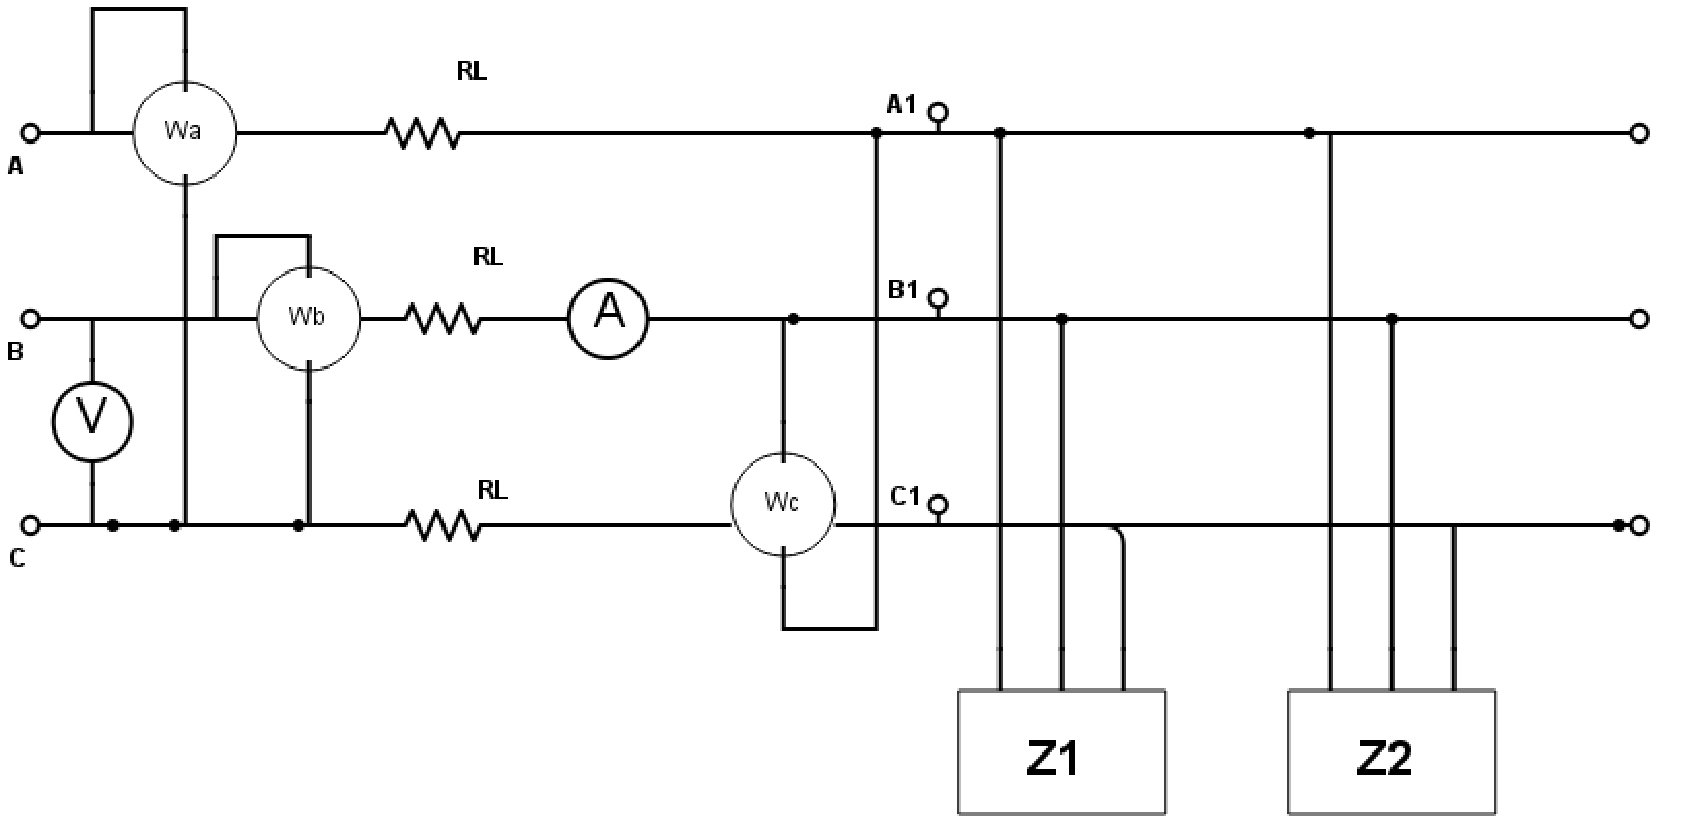
\includegraphics[scale=0.4]{figs/FiguraBT3.pdf}
\end{center}

\begin{enumerate}
\item Lectura del vatímetro $W_c$.
\item Lectura del amperímetro.
\item Factor de potencia total de las cargas (en retraso o
  adelanto).
\item Lectura de los vatímetros $W_a$ y $W_b$.
\item Lectura del voltímetro.
\item Valor de los condensadores conectados en $A_1B_1C_1$ para
  que el f.d.p. en ese punto sea la unidad.
\item Lecturas de los cinco aparatos de medida tras el apartado
  anterior.
\end{enumerate}

Datos:
\begin{itemize}
\item Secuencia de fases directa, $f = \SI{50}{\hertz}$, ($A_1B_1C_1$)
  $U_1 = \SI{420}{\volt}$.
\item $Z_1$: motor de 10 CV, con $\eta = 0.83$, y f.d.p. de 0'9.
\item $Z_2$: conjunto de iluminación fluorescente, con
  $P = \SI{2400}{\watt}$, y f.d.p. de 0'85.
\item $R_L = \SI{1}{\ohm}$.
\end{itemize}

\noindent\hrulefill

A partir de los datos del enunciado, teniendo en cuenta que las dos
cargas son inductivas, obtenemos:
\begin{align*}
  P_1 &= \SI{8867.5}{\watt}\\
  Q_1 &= \SI{4294.7}{VA}_r\\
  P_2 &= \SI{2400}{\watt}\\
  Q_2 &= \SI{1487.4}{VA}_r\\
\end{align*}
Por tanto, el triángulo de potencias de las cargas ($A_1B_1C_1$) es:
\begin{align*}
  P &= \SI{11267.5}{\watt}\\
  Q &= \SI{5782.1}{VA}_r\\
  S &= \SI{12664.5}{VA}\\
\end{align*}

Dado que se trata de un sistema de SFD, la lectura del vatímetro $W_c$
es:

\begin{equation*}
  W_c = - \frac{Q}{\sqrt{3}} = \SI{-3338.3}{\watt}
\end{equation*}

La lectura del amperímetro es:

\begin{equation*}
  A = \frac{S}{\sqrt{3} U} = \SI{17.41}{\ampere}
\end{equation*}

El factor de potencia de las cargas es:

\begin{equation*}
  fdp = \cos{\arctan{\frac{Q}{P}}} = 0.89
\end{equation*}

La potencia disipada en la línea es:

\begin{equation*}
  P_L = 3 \cdot I^2 \cdot R_L = \SI{909.32}{\watt}
\end{equation*}

Y, por tanto, el triángulo de potencias total es:

\begin{align*}
  P_T = P + P_L &= \SI{12176.8}{\watt}\\
  Q_T = Q &= \SI{5782.1}{VA}_r\\
  S_T &= \SI{13479.9}{VA}
\end{align*}

Teniendo en cuenta que:

\begin{align*}
  W_A + W_B &= P_T\\
  W_A - W_B &= Q_T / \sqrt{3}
\end{align*}

obtenemos

\begin{align*}
  W_A &= \SI{7757.6}{\watt}\\
  W_B &= \SI{4419.27}{\watt}
\end{align*}

La tensión a la entrada de la línea es:

\begin{equation*}
  U' = \frac{S_T}{\sqrt{3} I} = \SI{447.02}{\volt}
\end{equation*}

Los condensadores necesarios (conectados en triángulo) deben tener una
capacidad de:

\begin{equation*}
  C = \frac{Q_T}{3U^2\omega} = \SI{34.78}{\micro\farad}
\end{equation*}

Con estos condensadores conectados, las lecturas de los aparatos de
medida son:

\begin{align*}
  W_c &= 0\\
  A &= \SI{15.5}{\ampere}\\
  P_L &= \SI{720.75}{\watt}\\
  P_T &= \SI{11988.25}{\watt}\\
  W_A = W_B &= \SI{5994.1}{\watt}\\
  U' &= \SI{446.5}{\volt}\\  
\end{align*}

\clearpage

\section{}

Una línea ideal trifásica de 4 hilos alimenta a dos cargas a una
tensión de $\SI{400}{\volt}$ en secuencia de fases inversa (SFI) y
frecuencia $\SI{50}{\hertz}$.

Las cargas tienen las siguientes características:

\begin{itemize}
\item Un motor trifásico de $\SI{70}{\kilo\watt}$ y f.d.p. de 0.8.
\item Un conjunto equilibrado de 90 lámparas fluorescentes. Las
  características de cada lámpara son: potencia de $\SI{12}{\watt}$,
  f.d.p. de 0.7 en retraso, tensión $\SI{230}{\volt}$.
\end{itemize}

Con esta información se pide:

\begin{enumerate}
\item Conectar adecuadamente los siguientes aparatos de medida antes
  de las cargas.
  \begin{itemize}
  \item Un voltímetro que mida la tensión de línea (etiquetado como
    $V_L$) y otro voltímetro que mida la tensión de fase (etiquetado
    como $V_F$).
  \item Un vatímetro que permita calcular la potencia reactiva total
    del sistema (etiquetado como $W_r$).
  \item Dos vatímetros que, de forma conjunta, permitan calcular la
    potencia activa total del sistema (etiquetados como $W_X$ y
    $W_Y$).
  \end{itemize}
\item Calcular el valor eficaz de la corriente de línea
  total.
\item Calcular la lectura de cada uno de los aparatos
  de medida del primer apartado.
\item Calcular los condensadores necesarios para
  mejorar el factor de potencia hasta 0,9, indicando cómo se deben
  conectar.
\item vez conectados los condensadores del anterior
  apartado, determinar la corriente de línea y la lectura de todos los
  aparatos de medida del apartado 2.
\end{enumerate}

\noindent\hrulefill

El motor consume una potencia activa de $P_m = 70\mathrm{kW}$. Su
potencia reactiva es
$Q_m = P_m \cdot \tan(\theta_m) = 52.5\mathrm{kVAr}$.  Las lámparas
consumen una potencia activa de $P_f = 90 \cdot 12 =
1080\mathrm{W}$. Su potencia reactiva (inductiva) es
$Q_f = 1101.8\mathrm{VAr}$.  Aplicando Boucherot, la potencia activa
total es $P = P_m + P_f = 71.08\mathrm{kW}$ y la potencia reactiva
total es $Q = Q_m + Q_f = 53.6\mathrm{kVAr}$. Con estas magnitudes
podemos calcular el factor de potencia global, $\cos(\theta) =
0.798$. Finalmente, la corriente de línea es:

\[
  I = \frac{P}{\sqrt(3) \cdot U \cdot \cos(\theta)} = 128.5\mathrm{A}
\]


Teniendo en cuenta que es un sistema equilibrado y que es SFI,

\begin{itemize}

\item Para medir la tensión de línea hay que conectar un voltímetro
  entre dos fases. La medida será $V_{L} = 400\mathrm{V}$. Para medir
  la tensión de fase hay que conectar un voltímetro entre una fase y
  el neutro.$V_{AN} = 400 / \sqrt{3} = 230.9\mathrm{V}$

\item Hay que conectar un vatímetro midiendo tensión entre dos fases y
  la corriente por la tercera. Para que la medida coincida en signo
  con la de la potencia reactiva, la conexión entre fases debe ser BA,
  CB, o AC. Así, por ejemplo, un vatímetro midiendo tensión entre A y
  C, y corriente por B medirá $W_R = Q / \sqrt{3} = 30947\mathrm{W}$

\item Hay que usar el método de Aron. Una posibilidad es conectar un
  vatímetro midiendo tensión entre las fases A y C, y corriente en A
  ($W_X$), y otro vatímetro midiendo tensión entre las fases B y C, y
  corriente por B ($W_Y$). Para obtener la potencia activa total del
  sistema basta con sumar las dos medidas: $W_{X} + W_{Y} =
  P$. Además, podemos usar la diferencia para obtener la
  reactiva. Teniendo en cuenta que se trata de una SFI,
  $W_Y - W_X = Q/\sqrt{3}$. Por tanto, $W_X = \SI{20666.5}{\watt}$,
  $W_Y = \SI{51013.5}{\watt}$.

\end{itemize}


Serán necesarios tres condensadores conectados en triángulo en
paralelo con las cargas. Deben suministrar una potencia reactiva
$Q_c = P \cdot (\tan(\theta) - \tan(\theta')) = \SI{19176.2}{VAr}$

Por tanto, la capacidad de cada condensador es:

\[
  C = \frac{Q_c}{3 \cdot \omega \cdot U^2} = \SI{127.2}{\micro\farad}
\]

El sistema incluyendo los condensadores consume la misma potencia
activa. Por tanto, la corriente es ahora:

\[I' = \frac{P}{\sqrt{3} \cdot U \cdot cos(\theta')} = \SI{114}{A}\]

La potencia reactiva es ahora:

\[
  Q' = P \cdot \tan(\theta') = \SI{34425.62}{VAr}
\]

Los aparatos de medida descritos antes miden ahora:
\begin{itemize}
\item La medida de los voltímetros no cambia.
\item $W_X = \SI{25602.2}{W}$
\item $W_Y = \SI{45477.8}{W}$
\item $W_R = \SI{19875.6}{W}$
\end{itemize}


\end{document}





